\begin{enumerate}
\setcounter{enumi}{0}
    \item Sea una empresa dedicada al transporte y distribución de mercancías, la cual tiene una planilla de 50 trabajadores. Durante los últimos años se
ha observado que 25 trabajadores han faltado un solo dia al trabajo. 20 trabajadores han faltado2 días y 5 trabajadores han faltado 3 días. Si se toma una
muestra aleatoria simple con reemplazo, de tamaño 2 del total de la planilla.

    \begin{enumerate}[a)]
        \item La distribución de probabilidad del número de días que faltado al trabajo un empleado, su media y su varianza.
        \item Distribución de probabilidad del estadístico media muestral $\bar{X}$.
        \item Distribución de probabilidad del estadístico varianza muestral $S^2$.
        \item La media y varianza del estadístico media muestral.
        \item La probabilidad de que el estadístico media muestral, $\bar{X}$, sea menor que 2.
        \item La media y varianza del estadístico varianza muestral.
        \item La probabilidad de que el estadístico varianza muestral $S^2$, sea menor o igual a 0,5
    \end{enumerate}

    \\
    \textbf{Solución item A:}
    \\\\
    Sea  X  número de días que ha faltado un empleado elegido aleatoriamente de la plantilla total.
    
    \begin{lstlisting}[frame=single]
    x <- c(1, 2, 3)
    Px <- c('P(X=1)', 'P(X=1)', 'P(X=1)')
    pf <- c('25/50', '20/50', '5/50')
    p <- c(0.5, 0.4, 0.1)
    df2 <- data.frame(x, Px, pf, p)
    library(tidyverse)
    df2
    \end{lstlisting}
    \begin{verbatim}
    este es un comentario.
    \end{verbatim}
    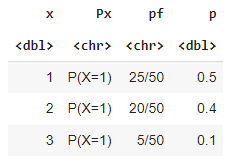
\includegraphics[scale=1]{img/tab1.png}
    \\
    \begin{lstlisting}[frame=single]
    ggplot(df2, aes(x, p))+geom_bar(stat="identity",width=0.5)
    \end{lstlisting}

    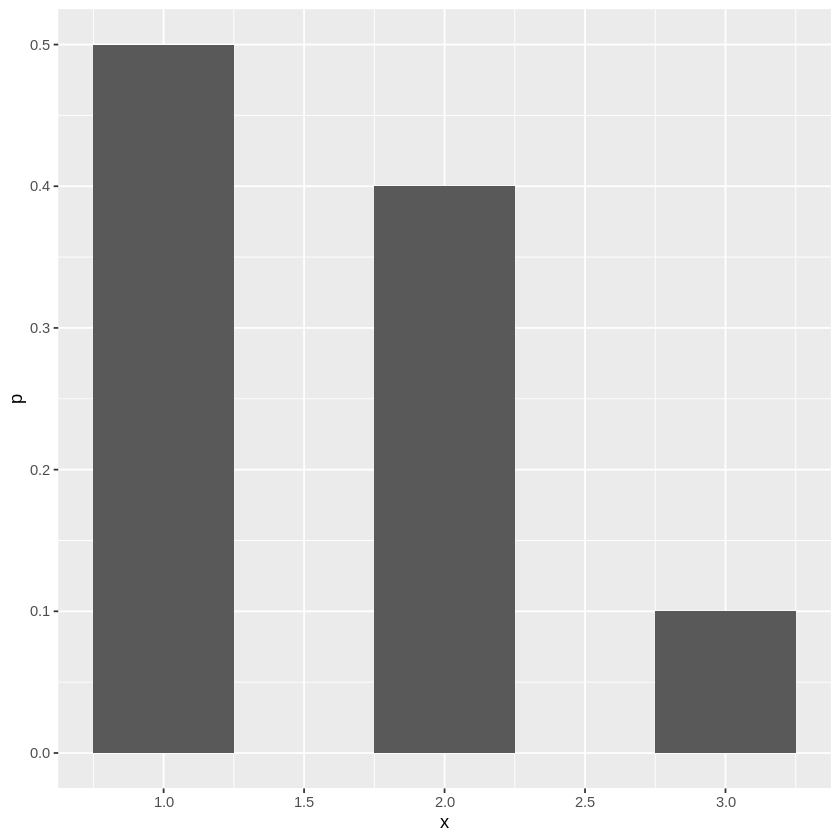
\includegraphics[scale=0.5]{img/tab2.png}
    
    \begin{lstlisting}[frame=single]
    media <- 0
    for (i in 1:3) {
      media <-media + (x[i] * p[i])
    }
    media
    \end{lstlisting}
    \begin{verbatim}
    1.6
    \end{verbatim}
    
    \begin{lstlisting}[frame=single]
    varianza <- 0
    for (i in 1:3) {
      varianza <-varianza + (p[i]*(x[i]-1.6)^2 )
    }
    varianza
    \end{lstlisting}
    \begin{verbatim}
    0.44
    \end{verbatim}
    

\end{enumerate}